\definecolor{Planung}{HTML}{FF1111}
\definecolor{Backend}{HTML}{00FFC1}
\definecolor{ACP}{HTML}{2F95DE}
\definecolor{Seite}{HTML}{299819}
\definecolor{Dokumentation}{HTML}{2300E7}

\section*{Arbeitsprotokoll - Alexander Bertoni}

\begin{table}[H]
    \begin{tabular}{lrr}
        \hline
        \textbf{Projekt} & \multicolumn{1}{l}{\textbf{Arbeitsaufwand}} & \multicolumn{1}{l}{\textbf{Prozent}} \\ \hline
        \fcolorbox{black}{Planung}{\rule{0pt}{4pt}\rule{4pt}{0pt}} Planung & 2:41:10 & 1.40\% \\
        \fcolorbox{black}{Seite}{\rule{0pt}{4pt}\rule{4pt}{0pt}} Seite & 153:25:45 & 79.78\% \\
        \fcolorbox{black}{Dokumentation}{\rule{0pt}{4pt}\rule{4pt}{0pt}} Dokumentation & 36:12:34 & 18.82\% \\
        \hline
        \textbf{Summe} & \textbf{192:19:29} & \textbf{100.00\%} \\
        \hline
    \end{tabular}
\end{table}

\begin{figure}[H]
    \begin{center}
        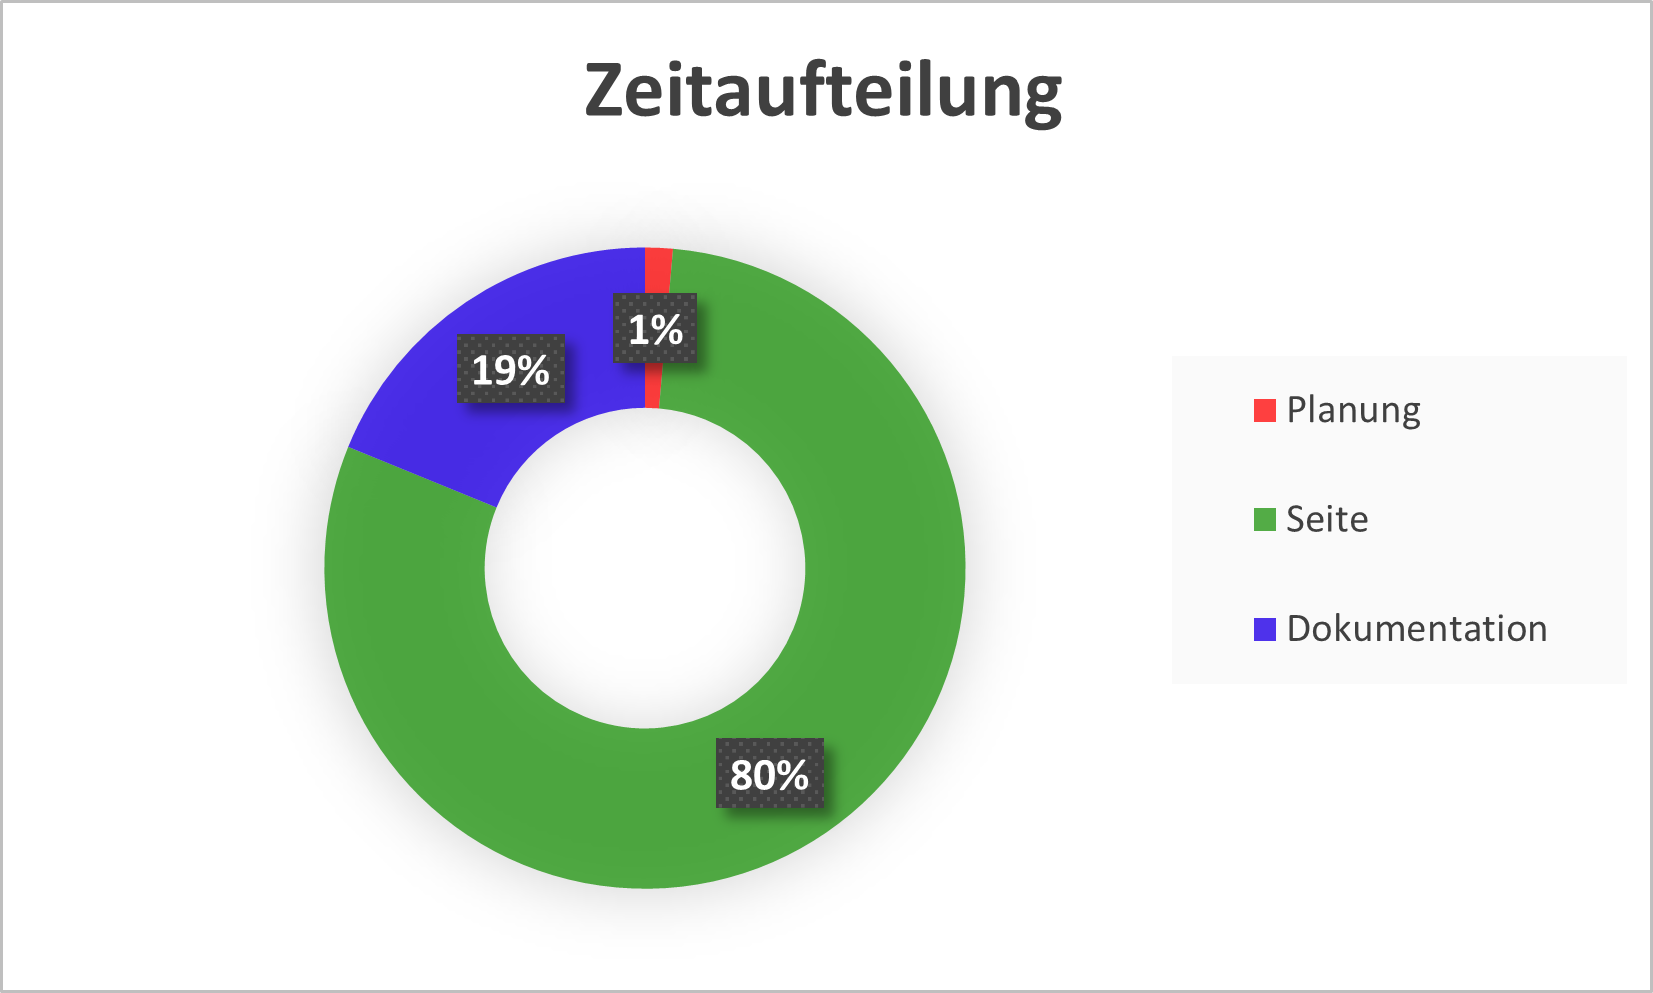
\includegraphics[width=1\textwidth]{images/Zeiten/Zeitaufteilung-Bertoni.png}
        \caption{Verteilung von Alexanders Arbeitsstunden}
    \end{center}
\end{figure}

\begin{figure}[H]
    \begin{center}
        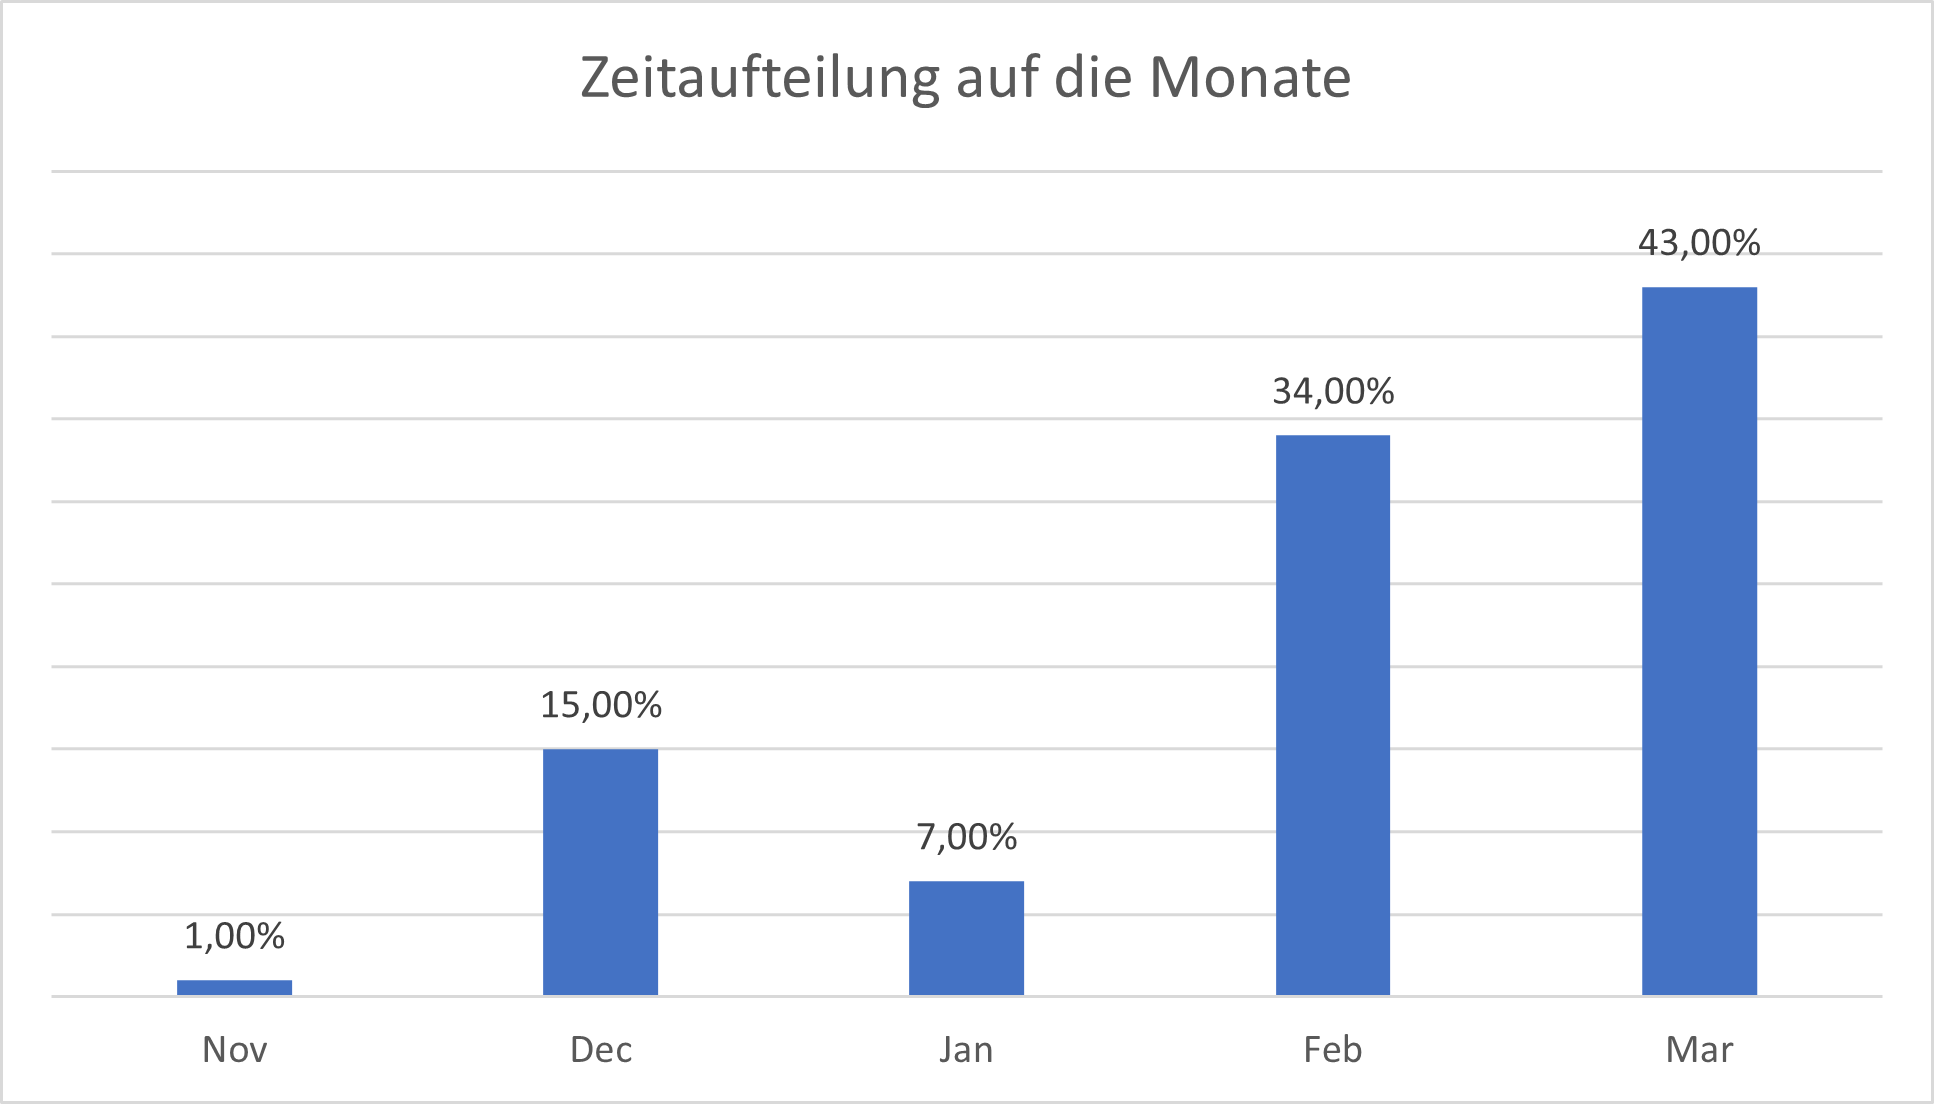
\includegraphics[width=1\textwidth]{images/Zeiten/Zeitaufteilung-auf-Monate-Bertoni.png}
        \caption{Alexanders Arbeitszeiten vom 07.12.2021 bis zum 20.03.2022}
    \end{center}
\end{figure}

\newpage
\section*{Arbeitsprotokoll - Philipp Schuler}

\begin{table}[H]
\begin{tabular}{lrr}
\hline
\textbf{Projektteil}  & \textbf{Arbeitsaufwand} & \textbf{Prozentueller Anteil} \\ \hline
Technologie erlernen  & 32:57:00                   & 17,16\%                    \\
Planung               &  7:31:12                   &  3,92\%                    \\
App Design und Aufbau & 48:35:25                   & 25,30\%                    \\
Funktionalität        & 75:25:09                   & 39,27\%                    \\
Dokumentation         & 27:34:50                   & 14,36\%                    \\ \hline
\textbf{Summe}        & \textbf{192:03:36}         & \textbf{100,00\%}             \\ \hline
\end{tabular}
\end{table}

\begin{figure}[H]
    \begin{center}
        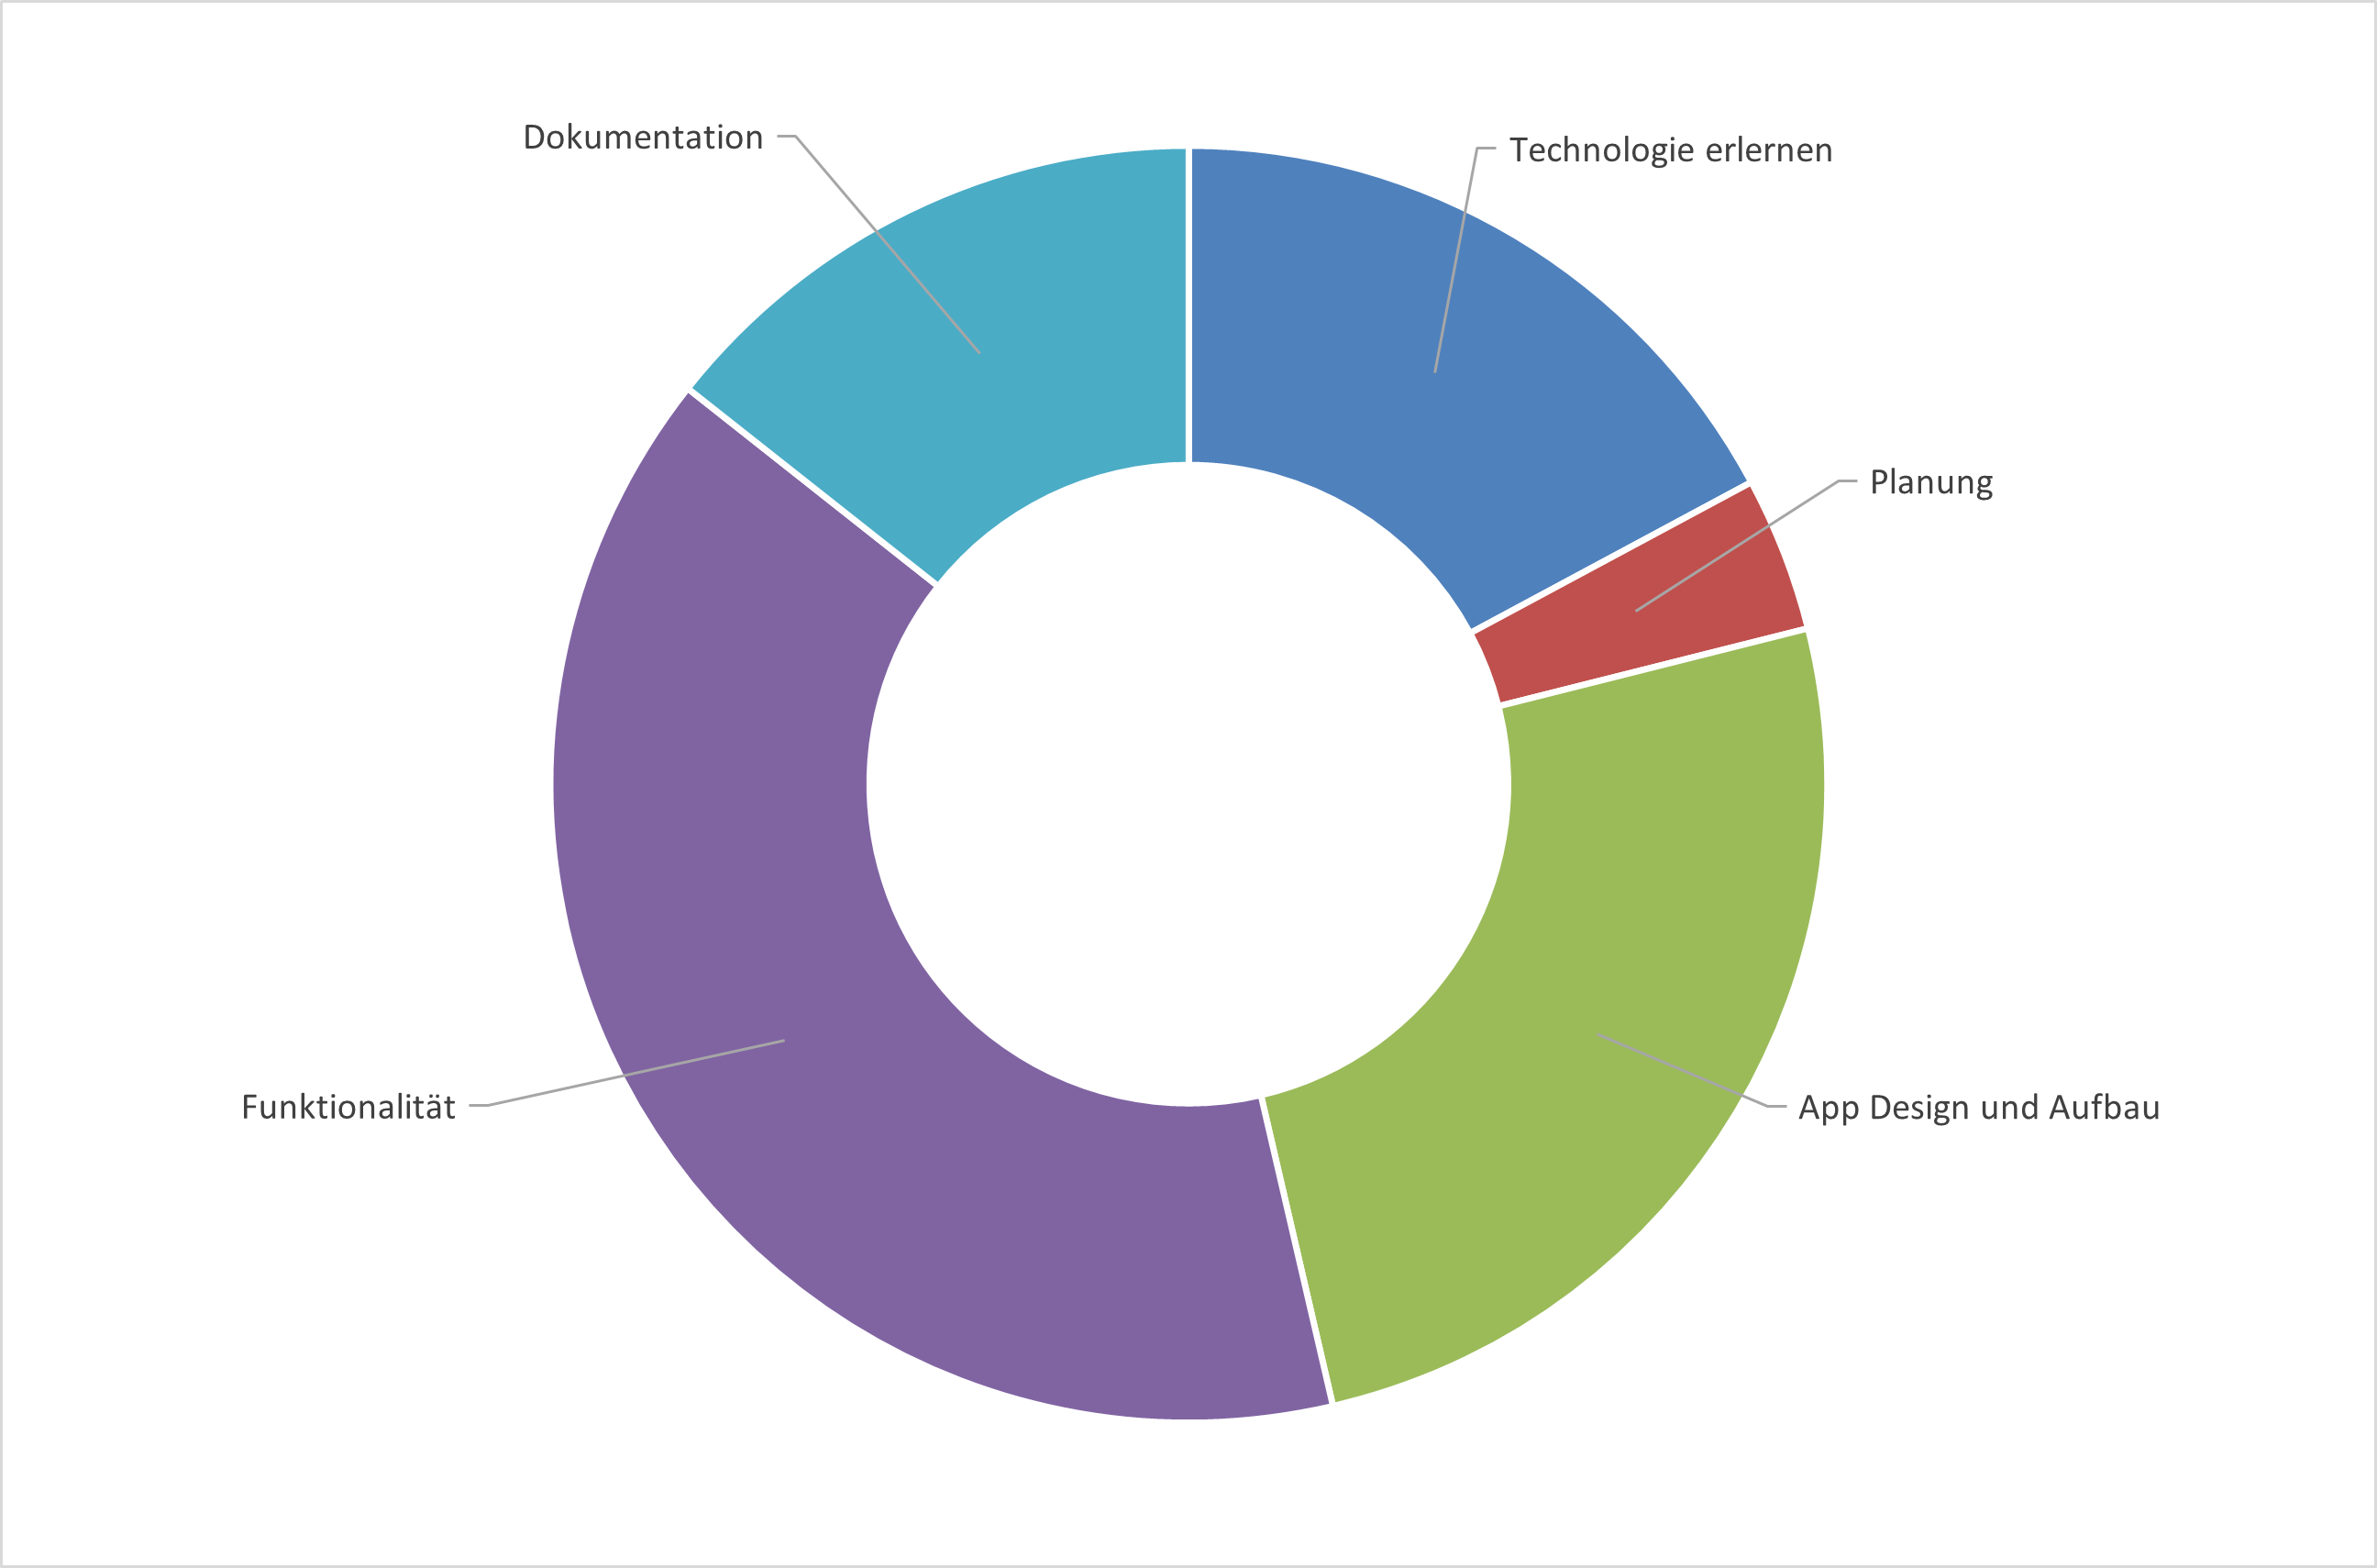
\includegraphics[width=0.8\textwidth]{Appendix/Philipp/Kuchen.png}
        \caption{Verteilung von Philipp's Arbeitsstunden}
    \end{center}
\end{figure}

\begin{figure}[H]
    \begin{center}
        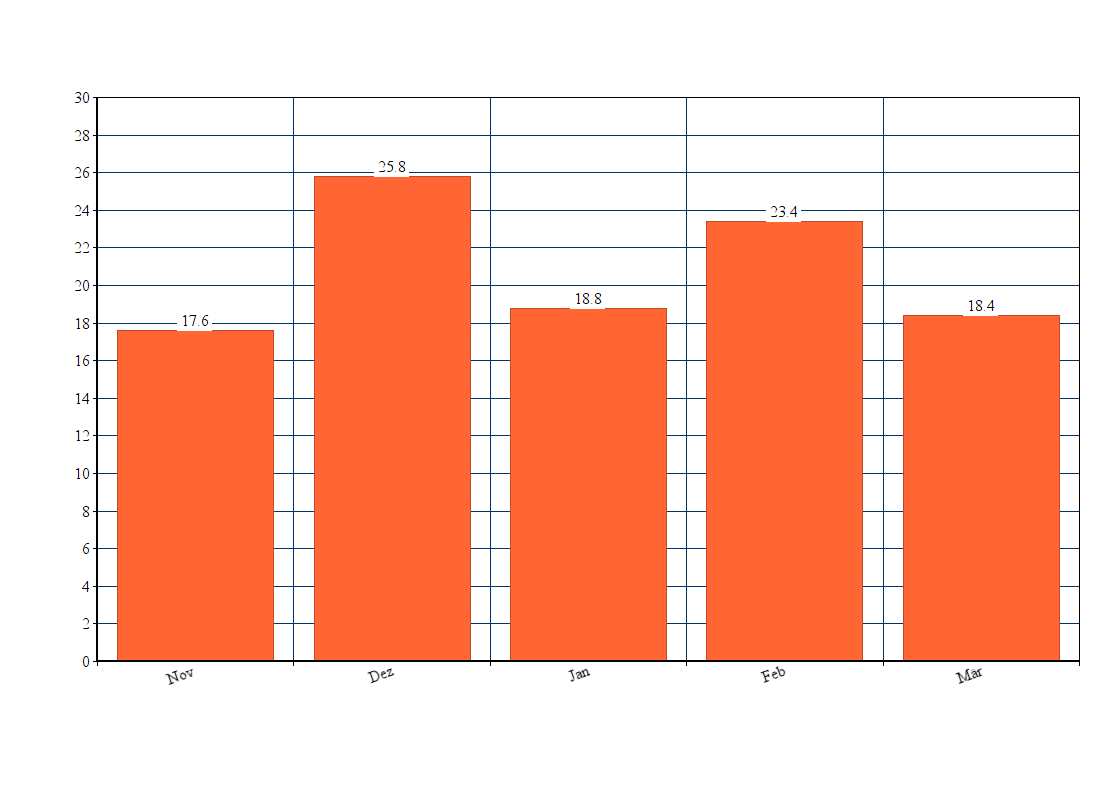
\includegraphics[width=1\textwidth]{Appendix/Philipp/Balken.png}
        \caption{Philipp's Arbeitsverlauf vom 30.11.2021 bis zum 20.03.2022}
    \end{center}
\end{figure}
